%%%%%%%%%%%%%%%%%%%%%%%%%%%%%%%%%%%%%%%%%
% Programming/Coding Assignment
% LaTeX Template
%
% This template has been downloaded from:
% http://www.latextemplates.com
%
% Original author:
% Ted Pavlic (http://www.tedpavlic.com)
%
% Note:
% The \lipsum[#] commands throughout this template generate dummy text
% to fill the template out. These commands should all be removed when 
% writing assignment content.
%
% This template uses a Perl script as an example snippet of code, most other
% languages are also usable. Configure them in the "CODE INCLUSION 
% CONFIGURATION" section.
%
%%%%%%%%%%%%%%%%%%%%%%%%%%%%%%%%%%%%%%%%%

%----------------------------------------------------------------------------------------
%	PACKAGES AND OTHER DOCUMENT CONFIGURATIONS
%----------------------------------------------------------------------------------------
\documentclass{article}

\usepackage{fancyhdr} % Required for custom headers
\usepackage{lastpage} % Required to determine the last page for the footer
\usepackage{extramarks} % Required for headers and footers
\usepackage[usenames,dvipsnames]{color} % Required for custom colors
\usepackage{graphicx} % Required to insert images
\usepackage{listings} % Required for insertion of code
\usepackage{courier} % Required for the courier font
\usepackage{pgfgantt}
\usepackage{amsmath}
\usepackage{mathabx}
\usepackage{mathtools}
\usepackage{qtree}
\usepackage{multicol}
\usepackage{fancyvrb}
\usepackage{setspace}
\usepackage{csquotes}




% Margins
\topmargin=-0.45in
\evensidemargin=0in
\oddsidemargin=0in
\textwidth=6.5in
\textheight=9.0in
\headsep=0.3in

\linespread{1.1} % Line spacing

% Set up the header and footer
\pagestyle{fancy}
\lhead{\homeworkProblemName} % Top left header
\chead{} % Top center head
\rhead{\hmwkClass} % Top right header
\lfoot{\textit{\homeworkSectionName}} % Bottom left footer
\cfoot{} % Bottom center footer
\rfoot{Page\ \thepage\ of\ \protect\pageref{LastPage}} % Bottom right footer
\renewcommand\headrulewidth{0.4pt} % Size of the header rule
\renewcommand\footrulewidth{0.4pt} % Size of the footer rule

\setlength\parindent{0pt} % Removes all indentation from paragraphs

%----------------------------------------------------------------------------------------
%	CODE INCLUSION CONFIGURATION
%----------------------------------------------------------------------------------------

\definecolor{MyDarkGreen}{rgb}{0.0,0.4,0.0} % This is the color used for comments
\lstloadlanguages{Java} % Load Java syntax for listings, for a list of other languages supported see: ftp://ftp.tex.ac.uk/tex-archive/macros/latex/contrib/listings/listings.pdf
\lstset{language=Java, % Use Java in this example
        frame=none, % Single frame around code
        basicstyle=\small\ttfamily, % Use small true type font
        keywordstyle=[1]\color{Blue}\bf, % Perl functions bold and blue
        keywordstyle=[2]\color{Purple}, % Perl function arguments purple
        keywordstyle=[3]\color{Blue}\underbar, % Custom functions underlined and blue
        identifierstyle=, % Nothing special about identifiers                                         
        commentstyle=\usefont{T1}{pcr}{m}{sl}\color{MyDarkGreen}\small, % Comments small dark green courier font
        stringstyle=\color{Purple}, % Strings are purple
        showstringspaces=false, % Don't put marks in string spaces
        tabsize=8, % 5 spaces per tab
        %
        % Put standard Perl functions not included in the default language here
        morekeywords={rand},
        %
        % Put Perl function parameters here
        morekeywords=[2]{on, off, interp},
        %
        % Put user defined functions here
        morekeywords=[3]{test},
       	%
        morecomment=[l][\color{Blue}]{...}, % Line continuation (...) like blue comment
        numbers=left, % Line numbers on left
        firstnumber=1, % Line numbers start with line 1
        numberstyle=\tiny\color{Blue}, % Line numbers are blue and small
        stepnumber=100 % Line numbers go in steps of 5
}


%----------------------------------------------------------------------------------------
%	DOCUMENT STRUCTURE COMMANDS
%	Skip this unless you know what you're doing
%----------------------------------------------------------------------------------------

% Header and footer for when a page split occurs within a problem environment
\newcommand{\enterProblemHeader}[1]{
\nobreak\extramarks{#1}{#1}\nobreak
\nobreak\extramarks{#1}{#1}\nobreak
}

% Header and footer for when a page split occurs between problem environments
\newcommand{\exitProblemHeader}[1]{
\nobreak\extramarks{#1}{#1 continued on next page\ldots}\nobreak
\nobreak\extramarks{#1}{}\nobreak
}

\setcounter{secnumdepth}{0} % Removes default section numbers
\newcounter{homeworkProblemCounter} % Creates a counter to keep track of the number of problems

\newcommand{\homeworkProblemName}{}
\newenvironment{homeworkProblem}[1][
 \arabic{homeworkProblemCounter}]{ % Makes a new environment called homeworkProblem which takes 1 argument (custom name) but the default is "Problem #"
\stepcounter{homeworkProblemCounter} % Increase counter for number of problems
\renewcommand{\homeworkProblemName}{#1} % Assign \homeworkProblemName the name of the problem
\section{\homeworkProblemName} % Make a section in the document with the custom problem count
\enterProblemHeader{} % Header and footer within the environment
}{
\exitProblemHeader{} % Header and footer after the environment
}

\newcommand{\problemAnswer}[1]{ % Defines the problem answer command with the content as the only argument
\noindent\framebox[\columnwidth][c]{\begin{minipage}{0.98\columnwidth}#1\end{minipage}} % Makes the box around the problem answer and puts the content inside
}

\newcommand{\homeworkSectionName}{}
\newenvironment{homeworkSection}[1]{ % New environment for sections within homework problems, takes 1 argument - the name of the section
\renewcommand{\homeworkSectionName}{#1} % Assign \homeworkSectionName to the name of the section from the environment argument
\subsection{\homeworkSectionName} % Make a subsection with the custom name of the subsection
\enterProblemHeader{\homeworkProblemName\ [\homeworkSectionName]} % Header and footer within the environment
}{
\enterProblemHeader{\homeworkProblemName} % Header and footer after the environment
}

%my commands
\newcommand{\dent}{\qquad\qquad}


%----------------------------------------------------------------------------------------
%	NAME AND CLASS SECTION
%----------------------------------------------------------------------------------------

\newcommand{\hmwkTitle}{Final Year Project Report} % Assignment title
\newcommand{\hmwkDesc}{A thesis submitted in part fulfilment of the degree of\\
\textbf{BSc. (Hons.) in Computer Science}} % Due date
\newcommand{\hmwkClass}{A Theorem Proving Assistant} % Course/class
\newcommand{\hmwkClassTime}{} % Class/lecture time
\newcommand{\hmwkClassInstructor}{Interim Report} % Teacher/lecturer
\newcommand{\hmwkAuthorName}{Joe Duffin} % Your name

%----------------------------------------------------------------------------------------
%	TITLE PAGE
%----------------------------------------------------------------------------------------

\title{
\vspace{0.3in}
\textbf{\hmwkTitle}
\vspace{1in}\\
\textmd{\textbf{\hmwkClass}}\\\ \\
\normalsize\
\vspace{0.4in}
\textmd{\textbf{\hmwkAuthorName}}\\
\vspace{0.1in}
\small{\hmwkDesc}\\
\vspace{0.05in}
\small{\textbf{Supervisor}: Henry Mcloughlin}
\vspace{.5in}
\begin{center}

\includegraphics[width=0.3\columnwidth]{UCD_Logo} % Example image
\end{center}
}


\author{School of Computer Science\\University College Dublin}


\date{\small{November 5, 2016}} % Insert date here if you want it to appear below your name

%use dash as list marker
\def\labelitemi{--}
%----------------------------------------------------------------------------------------

\begin{document}
\begin{titlepage}
\maketitle
\thispagestyle{empty}
\end{titlepage}

\newpage
%----------------------------------------------------------------------------------------
%	TABLE OF CONTENTS
%----------------------------------------------------------------------------------------

%\setcounter{tocdepth}{1} % Uncomment this line if you don't want subsections listed in the ToC

\newpage
\doublespacing
\tableofcontents
\singlespacing
\newpage

%----------------------------------------------------------------------------------------
\begin{homeworkProblem}[Project Specification]
\begin{description}

\item \textbf{General Information}\\
Calculational Theorem Proving is the name given to a particular style of mathematical proof which
was developed during the 1980s by Feijen and Dijkstra. It emphasises the syntactic manipulation
of expressions rather than manipulation based on an interpretation of the expression. In doing so it tries to let the notation do the work.\\

In order to do so the choice of notation and they layout of the proofs are important.\\

This style of proof has been taught in a number of our undergraduate modules over the last 10
years and is probably quite familiar to all of our undergraduates. An example proof would have
been included here but the special symbols for the boolean operators were not available.\\

The aim of this project is to develop a tool which will assist the person proving the theorem
by performing basic housekeeping tasks. So for example, the user should be able to select a
sub-expression, select an appropriate rule to transform it, and have the system carry out the
transformation and record the appropriate hint to show which rule was used and what the variable bindings were. It is important to mention that we are not interested in automatic theorem proving, the user will still be required to drive the proof but the system will perform the matching and applying of the rules.\\

It should be possible to store and retrieve partial or complete proofs. It should be possible to undo a series of steps and select different rules to apply. Once a theorem is proved it should be possible to add it to the rule base so it can be used in future proofs.

\item \textbf{Mandatory Requirements}\\
$\circ$ The design of algorithms to a selected sub-expression with a subexpression of a rule.\\
$\circ$ The design of an interface to allow users to select subexpressions and rules to apply.\\
$\circ$ The design of appropriate algorithms to allow partial and complete proofs to be stored and retrieved.\\
$\circ$ The design of appropriate algorithms to allow the user to undo steps in a proof.\\
$\circ$ The implementation of the above functionality.

\item \textbf{Discretionary Requirements}\\
$\circ$ Incorporating quantified expressions and their manipulation rules in the system.

\item \textbf{Exceptional Requirements}\\
$\circ$ Incorporating additional small calculii such as Max/Min, Floor/Ceiling and GCD/LCM into the system.

\item \textbf{Suggested Reading}\\
$\circ$ http://www.cs.utexas.edu/~EWD/\\
$\circ$ http://www.mathmeth.com/\\
$\circ$ Program Construction by Roland Backhouse\\
$\circ$ A logical approach to discrete maths by David Gries
\end{description}

\newpage
\end{homeworkProblem}
%----------------------------------------------------------------------------------------

\begin{homeworkProblem}[Abstract]

\begin{description}
\item \textbf{Context}\\
This report introduces the reader to predicate calculus and theorem proving in the style used by Dijkstra. It highlights the features of it that lend themselves to a computer application. Proving boolean theorems is a pattern matching excersise without need for interpretation of the expression at each stage of the proof. This report explores issues and solutions for building a software package which facilitates theorem proving in a clear and easy manor. A software package written in Java is presented from both user experience and technical development points of view.

\item \textbf{Methodology}\\
An exploratory approach was taken to not only resolving the major issues but finding them aswell. There is no road map to follow so a lot of time and resources were put into paths that led nowhere. In order to carry out this project algorithms were defined which were relied upon throughout, some of which have proven to be flawed and others invaluable. These will be discussed. A modular approach was taken to the software development, focusing compleleting small tasks and proving their correctness before moving on to the next.

\item \textbf{Findings}\\
Several major algorithms were defined to carry out the steps needed for theorem proving with the assistance of software. These algorihtms were implemented in Java and a fully functioning software package was produced. It facilitates theorem proving over the predicate calculus with quantified expressions as well as other small calculii such as max/min and floor/ceiling.

\end{description}

\newpage
\end{homeworkProblem}

%----------------------------------------------------------------------------------------

\begin{homeworkProblem}[Acknowledgments]
Thank you kindly
\newpage
\end{homeworkProblem}

%----------------------------------------------------------------------------------------

\begin{homeworkProblem}[Introduction]

As a race of humans it's in our very nature to look for connections and patterns. As soon as we see something we can associate with we grab onto it, we see where further expoloration of it will take us. When we compare the capabilities of humans with that of a matchine it is clear that machine wins in terms of raw processing power. When we attempt to compare this raw proccesing power to intelligence a strange divide occurs. It was only when an IBM computer (Deep Blue) was taught more patterns than a chess grand-master that it became "smarter" \cite{DEEPBLUE:1997}.

\begin{displayquote}
"Quite simply, humans are amazing pattern-recognition machines. They have the ability to recognize many different types of patterns - and then transform these  'recursive probabalistic fractals' into concrete, actionable steps."\cite{PROBFRACT}
\end{displayquote}

This report documents a software package called The Theorem Proving Assistnat. Its key feature is pattern matching. It can be used to prove boolean and arithmetic theorems not by evaluating the value of the expression but by comparing the expression to known truths. Importantly, matching the shape (or pattern) of an expression with known truths.\\

If I tell you $x+y$ is that same as $y+x$, or more formally $[x + y \equiv y + x]$ then what can you tell me about $p + q$? It's the same as $q + p$; clearly. However, attempting to define the simple logical steps you would need to instruct a computer perform this pattern matching operation is far from clear. What about $w+(p \times q)$? Clearly it's the same as $(p \times q)+w"$. At this point the problem has revealed it's extra dimensions. Are you going to list every possible combination? That's impossible. It's in our nature to solve these pattern related problems, a computer on the other hand, in this context, is stupid as hell without proper clear instruction.\\

This report also documents the algorithms devised and implemented to interpret these "recursive probabilisitic fractals" in such a way that pattern matching can be performed by a software package. These algorithms capture the essence of pattern matching as performed by a human to facilitate theorem proving in a fast, comprehensive and most importantly correct environment.

\newpage
\end{homeworkProblem}

%----------------------------------------------------------------------------------------
\begin{homeworkProblem}[Introduction to Dijykstra's Theorem Proving Style]
Predicate calculus theorem proving works like this: given a set of axioms and theorems (rules) one can calculate, or derive, further theorems. Relying on those derived previously a full calculus can be evolved. This process relies heavily on pattern matching and this notion is vitaly important. With each step of a proof a hint is given which tells the reader which rule was used and what assignment was made to each variable in that rule. Dijykstra states that the notation used is vitally important for a clear and easy to read proof \cite{DIJKSTRA:1990}.\\
\begin{homeworkSection}{Prelimniaries}
Before giving an example proof over the boolean domain we must set some conventions for notation and give information about operators. 
\begin{itemize}
\item Upper case letters such as $X$,$Y$ and $Z$ will be used as boolean identifiers.
\item For this brief introduction I am only going to introduce 3 operators:
\begin{description}
\item \textbf{Conjunction } - boolean multiplication: $\wedge$ reads as "and".
\item \textbf{Disjunction } - boolean addition: $\vee$ reads as"or".
\item \textbf{Equivalence } - boolean equals: $\equiv$ reads as "equival".
\end{description}
\item Equivalence holds the lowest precedence of the three operators and conjunction and disjunction share equal precedence meaning explicit bracketing must sometimes be used.
\item Brackets can be introduced as long as precedence and operators operands are respected.
\item Brackets can be removed under the same conditions as removal.
\item Rules will be numbered and named and be referenced to by their number or name.
\item Each new line of a proof will be preceeded by an assignment and the corresponding rule. We call this "the hint".\\
eg. $\{(X,Y\coloneqq Z,Y).(5)\}$ reads as $X$ and $Y$ are assigned the values $Z$ and $Y$ respectively in rule 5.
\item Axioms will be denoted with a $*$ to the left of it's number and theorems with a $\cdot$.
\end{itemize}
\vspace{0.5cm}
In order to give a sample proof I provide the following set of axioms and theorems.
\begin{align*}
&*\ (0)\ [(X\equiv (Y\equiv Z))\equiv ((X\equiv Y)\equiv Z)]&\equiv \text{ associative}\\
&*\ (1)\ [X\equiv Y\equiv Y \equiv X]&\equiv \text{ symmeetric}\\
&*\ (2)\ [X \equiv true \equiv X ]&\equiv \text{ identity}\\
&\cdot\ (3)\ [X \equiv X]&\equiv \text{ reflexive}\\
&\cdot\ (4)\ [true]&\text{true}\\
&*\ (5)\ [X \vee Y \equiv Y \vee X]&\vee \text{ symmetric}\\
&*\ (6)\ [X \vee (Y\vee Z) \equiv (X\vee Y) \vee Z]&\vee \text{ associative}\\
&*\ (7)\ [X \vee X \equiv X]&\vee \text{ idempotent}\\
&*\ (8)\ [X \vee (Y \equiv Z) \equiv X \vee Y \equiv X \vee Z]&\vee /\equiv 
\end{align*}
\newpage
\end{homeworkSection}

\begin{homeworkSection}{A Sample Proof}
We will now attempt to prove that disjuntion distributes over its self.
\begin{align*}
&(X\vee Y) \vee (X \vee Z) \\
\equiv&\dent \{(X,Y,Z\coloneqq (X\vee Y),X,Z).(6)\}\\
&((X\vee Y) \vee X) \vee Z \\
\equiv&\dent \{(X,Y\coloneqq (X\vee Y),X)).(5)\}\\
&(X \vee (X\vee Y)) \vee Z \\
\equiv&\dent \{(X,Y,Z\coloneqq (X,X,Y).(6)\}\\
&((X \vee X)\vee Y) \vee Z \\
\equiv&\dent \{(X\coloneqq X).(7)\}\\
&((X)\vee Y) \vee Z \\
\equiv&\dent \{remove\ brackets\}\\
&(X\vee Y) \vee Z \\
\equiv&\dent \{(X,Y,Z\coloneqq (X,Y,Z).(6)\}\\
&X\vee (Y \vee Z)\\
\end{align*}
This  has yielded a new theorem so we shall record it so it is available for use in future proofs.
\begin{align*}
&\cdot\ (9)\ [(X \vee Y) \vee (X \vee Z) \equiv X\vee (Y \vee Z)]&\vee/\vee
\end{align*}
Note that in the above proof no interpretation of any of the boolean expressions was done. It is purely a pattern matching exercise. At each step of the proof we used a single theorem to replace a section of an expression with an equivalent section. The theorem proving assistant functions by exploiting this feature of the proof style.\\

A second proof is provided here for demonstration. It proves that $P \vee true \equiv true$.
\begin{align*}
&P \vee true \\
\equiv&\dent \{(X:\coloneqq P).(2)\} \\
&P \vee ( P \equiv P ) \\
\equiv&\dent \{(X,Y,Z\coloneqq P,P,P ).(6)\} \\
&P \vee P \equiv P \vee P \\
\equiv&\dent \{(X \coloneqq P).(7)\} \\
&P \equiv P \vee P \\
\equiv&\dent \{(X \coloneqq P).(7)\} \\
&P \equiv P \\
\equiv&\dent \{(X \coloneqq P).(2)\} \\
& true
\end{align*}
Again we record the proof:
\begin{align*}
&\cdot\ (10)\ [P \vee true \equiv true] & \vee zero
\end{align*}
\newpage
\end{homeworkSection}

\begin{homeworkSection}{Further Notation and Calculii}
The brief above introduction uses three operators, conjunction, disjunction and equivalance. Dijykstra's theorem proving style holds for many other operators and even other calculii. Those that are important for comprehension of this report and available for use in the Theorem Proving Assistant are described below.
\begin{description}
\item \textbf{Other Boolean Operators}\\
Negation - $\neg$ \\
Implication - $\Rightarrow$ \\
Follows from  -  $\Leftarrow$ \\
Not Equivalent - $\not\equiv$ 

\item \textbf{Quantified Expressions}\\
Quantified expressions are a way of gathering boolean expressions with the same operator, either conjunction or disjunction. They consist of 3 parts seperated by colons.
\begin{enumerate}
 \setlength\itemsep{0em}
\item The quantifier and dummy
\item The range
\item The term
\end{enumerate}
The entire expression is wrapped in open-angled brackets as demonstrated in the examples below.
\begin{align*}
&\langle \forall i : r.i : f.i \vee X \rangle \text{ - For all i in the range r.i, f.i or X holds}\\
&\langle \exists j :: g.j \rangle \text{ - There exists a j in all ranges where g.j holds}
\end{align*}

\item \textbf{The Floor/Ceiling Calculus}\\
The floor/ceiling calculii are defined over the real numbers. The floor function rounds a number down to the next nearest integer and the ceiling function rounds a number up to the next nearest integer.
\begin{itemize}
\setlength\itemsep{0em}
\item Floor of x: $\lfloor x \rfloor$
\item Ceiling of x: $\lceil x \rceil$
\end{itemize}


\item \textbf{The Max/Min Calculus}\\
The max and min calculii are also defined over the real numbers. The max function yields the greater of it's two operands and the min function yields the lesser.
\begin{itemize}
\setlength\itemsep{0em}
\item Max of x and y: $x \uparrow y$
\item Min of x and y: $x \downarrow y$
\end{itemize}

\item \textbf{Lattice Theory}\\
I have no clue what to write :/


\end{description}
\newpage
\end{homeworkSection}

\end{homeworkProblem}
%----------------------------------------------------------------------------------------
\begin{homeworkProblem}[Introduction to The Theorem Proving Assistant]

\begin{homeworkSection}{The Software}
The theorem proving assistant is a user friendly software environment for assisting in proving predicate calculus theorems. It is not be an automated tool, but one which provides the user with a comprehensive and robust environment in which theorems can be proved. The software takes care of the "housework", such as automating the generation of the hint between each step.\\

The user is presented with an environment in which they prove theorems. To start a theorem the user needs an expression to work from. This is typed in in a plain text psuedo language (see Appendix A) and after clicking start a parser will transform the input into the correct form. For example: "X and Y" will be transformed into the expression "$X \wedge Y$".\\

The expression which the user is working with at any one time will be refered to as the current expression.  In order to carry out steps of the proof the following steps are carried out by the user:
\begin{enumerate}
\item Select a sub-expression in the current expression (the software ensures that only a valid subexpression can be chosen).
\item Choose a theorem to apply.
\item Make a selection of which replacement and assigment to use from a list of options.
\item View the new expression generated with a hint step describing which theorem and what assigment was used.
\item Continue to carry out steps with the new expression as the current expression until a conclusion has been drawn.
\item Save the proven theorem as a new theorem for future use.
\end{enumerate}

Further functionality allows the user to add and remove brackets where appropriate, undo a step, clear the work area and load or save theorem sets.
\newpage
\end{homeworkSection}

\begin{homeworkSection}{The Interface}
The interface consits of three distinct areas. The left hand side is refered to as the work area. It is here where the current expression and all steps taken to derive it are displayed. It in this area that a user will select a sub-expression of the current expression as described in step 2 above.\\

The righthand side of the interface will constists of both an area where a list of numbered theorems are displayed and also an area for replacement options to be displayed. The list of theorems will be made up of loaded axioms as well as theorems that have been previously prooved and saved by the user. It is here that a theorem will be chosen as described in step 3 above and the replacement options generated will be displayed in the options area. The user also has the ability to explore a theorem by clicking on it when the work area is clear. This "exploration" shows the theorems derivation which documents the steps taken in order to proove it as well as giving the option to either delete a theorem or continue work on it.\\

The 3 areas are surrounded by several buttons as well as the input box for generating the starting step of a proof. The buttons are used to access the functionality of the theorem proving assistant. If the use of a button is not appropriate at a given time, that buttons functionality is switched off.\\

\begin{center}
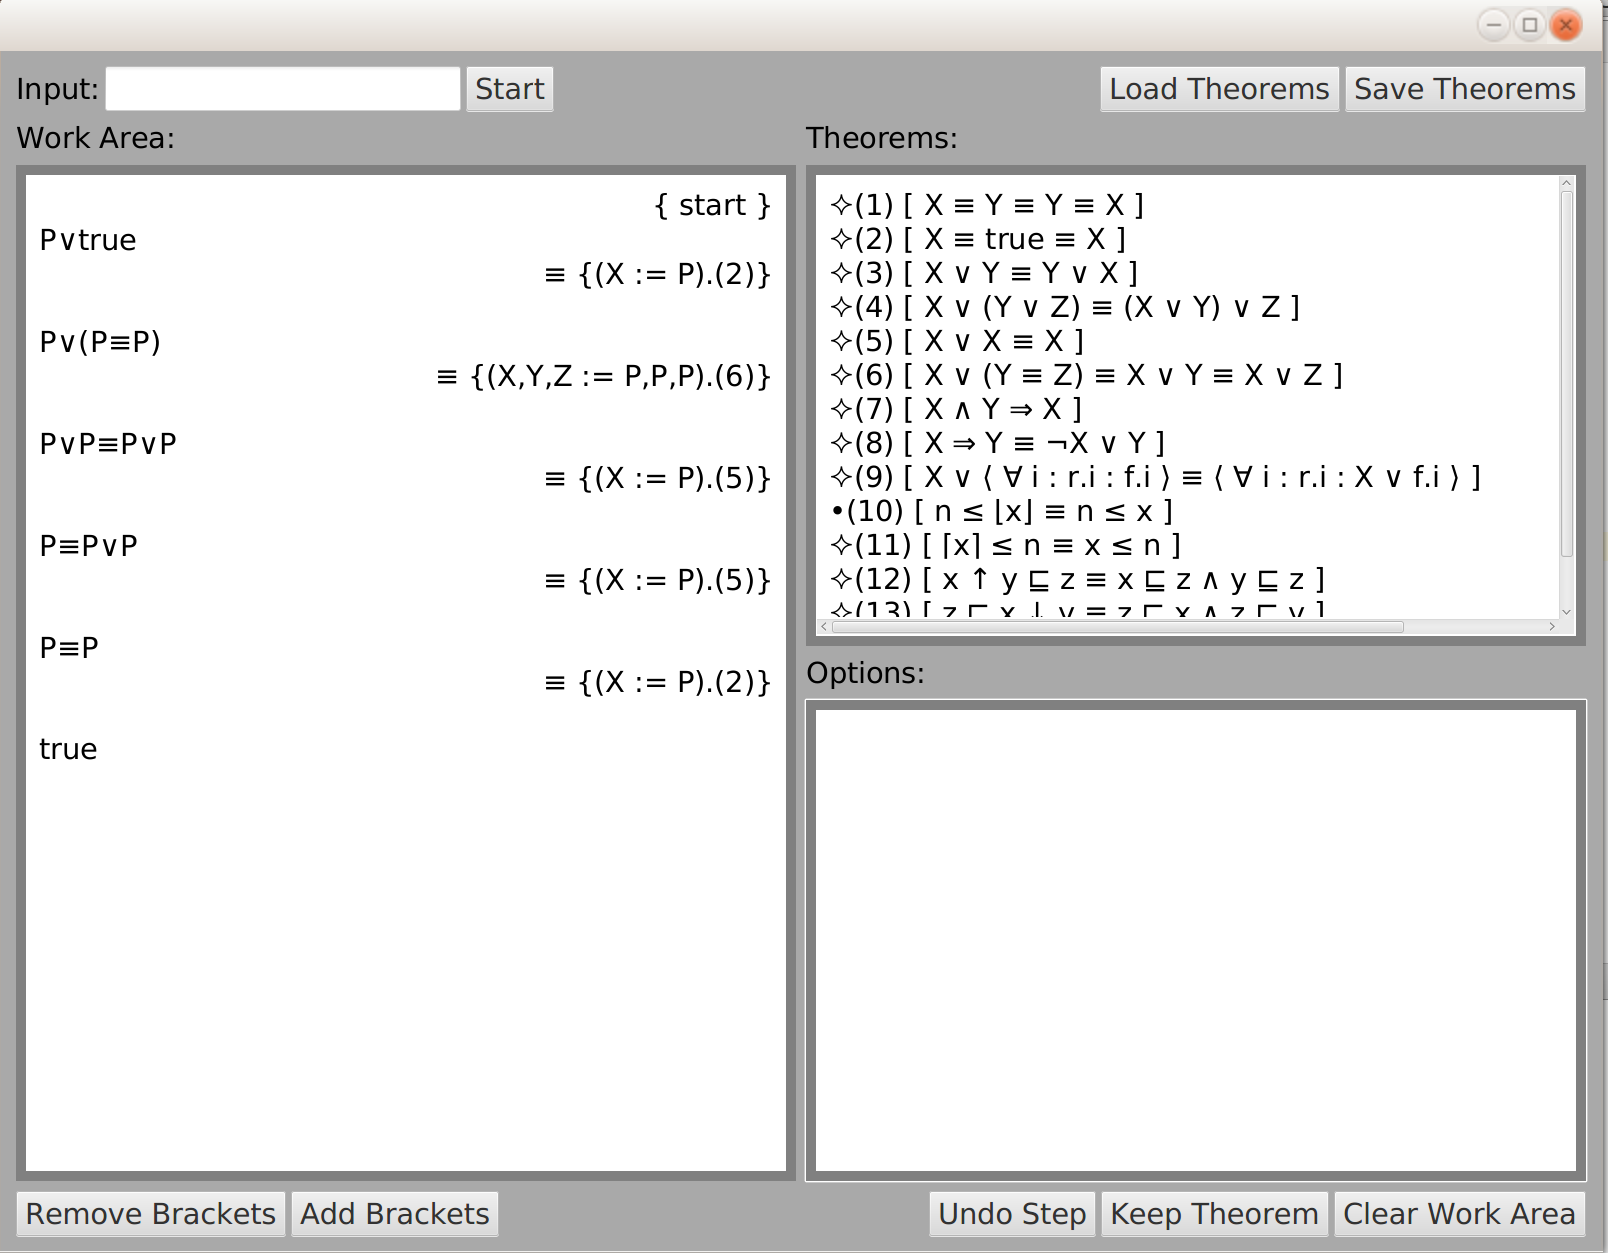
\includegraphics[width=1\columnwidth]{../screenshot} % Example image
\end{center}
\newpage
\end{homeworkSection}



\end{homeworkProblem}


%----------------------------------------------------------------------------------------
\begin{homeworkProblem}[Functionality Overview]

In this section the functionality of the Theorem proving assistant is explained. The steps are demonstrated with varying calculii to illustrate the versitility of the Theorem Proving Assistant.

\begin{homeworkSection}{Creating/Loading a Theorem Set}
Theorem files are stored in a JSON format but can be added to or created by writing theorems in the plain text psuedo-language (see Appendix A). A $*$ or a $-$ is used to indicate whethere this theorem should be interpretted as an axiom or not. Each theorem is placed on a seperate line and the software will automatically handle their indexes. For example, if the user wants to use boolean theorems relating to the Floor/Ceiling calculus the following would be added to a theorem file.
\begin{center}
\begin{minipage}{8cm}
\begin{Verbatim}[frame=single]
- |_ x _| < n == x < n
- x < |_ x _| + 1
- |_ x _| <= x and x < |_ x _| + 1
- |_ x _| <= |_ y _| <- x <= y
\end{Verbatim}
\end{minipage}
\end{center}


 After clicking the Load Theorems button and selecting the file the theorems will be loaded into the theorems area.
 
\begin{center}
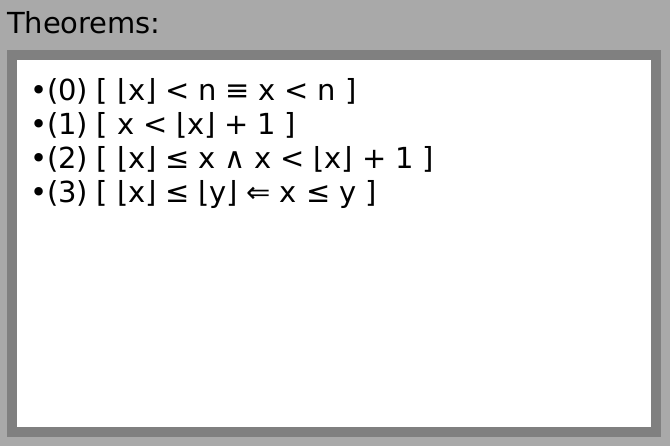
\includegraphics[width=0.4\columnwidth]{theoremload} 
\end{center}


\end{homeworkSection}
\begin{homeworkSection}{Starting a Proof}
To start a proof the user types the starting expression into the input box in plain text. The following example is taken from the Max/Min calculus.

\begin{center}

\includegraphics[width=0.3\columnwidth]{input} 
\end{center}

After clicking Start the input is parsed and presented to the user as the first proof step.

\begin{center}
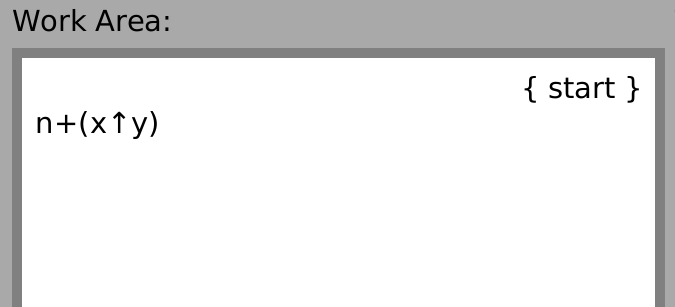
\includegraphics[width=0.4\columnwidth]{parsed} 
\end{center}
\newpage
\end{homeworkSection}

\begin{homeworkSection}{Performing a Proof Step}
To perform a proof step there are 3 distinct operations. This example demonstrates permuting a boolean term within a quantified expression.
\begin{description}

\item \textbf{Select A subexpression}\\
To select valid sub-expressions the user needs to select the operator around which the expression pivots. This is the lowest precedence operator in the required sub-expression. If multiple option are available, clicking multiple times will cycle the selection. Below shows the highlighting of several sub-expressions within the current expression.

\begin{center}
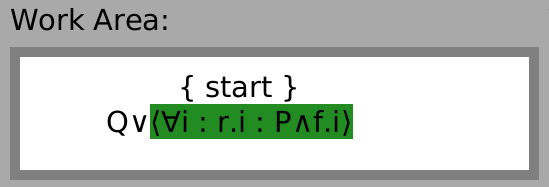
\includegraphics[width=0.4\columnwidth]{selection1} \qquad 
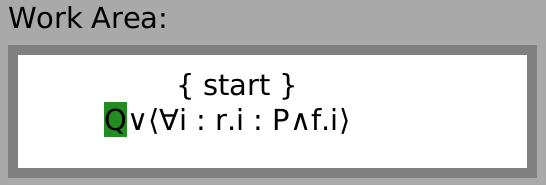
\includegraphics[width=0.4\columnwidth]{selection2} \\\ \\
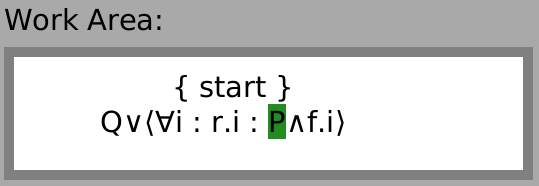
\includegraphics[width=0.4\columnwidth]{selection3} \qquad
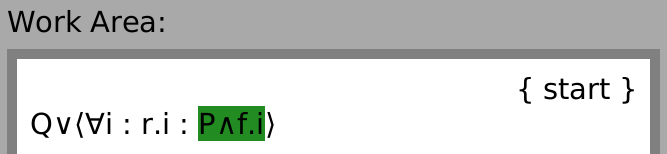
\includegraphics[width=0.4\columnwidth]{selection4} 
\end{center}

\item \textbf{Select A Theorem}\\
After choosing a sub-expression the user then needs to choose the theorem that they wish to apply. In this case we wish to commute $P$ and $f.i$ around the $\wedge$ operator so we choose rule $(0)$.

\begin{center}
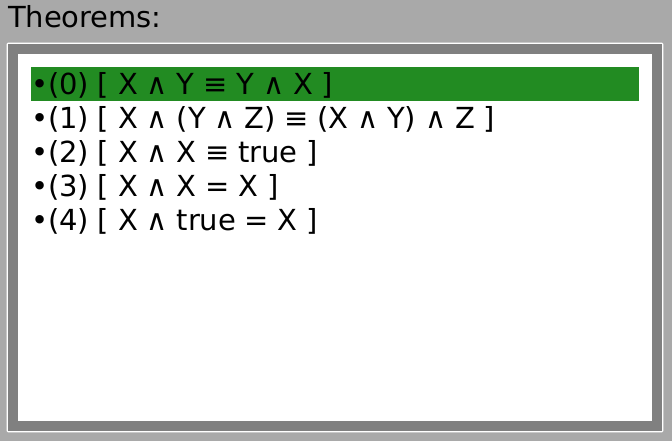
\includegraphics[width=0.4\columnwidth]{selectTheorem} 
\end{center}

\item \textbf{Select An Option}\\
The list of options is automatically generated after clicking a theorem. Each option shows what the new current expression will be along with the hint which informs the user of the assignment and the rule used.  In this case, after choosing theorem $(0)$ only two options are available. They both yield the same end result but the assignment in the hint is different. 

\begin{center}
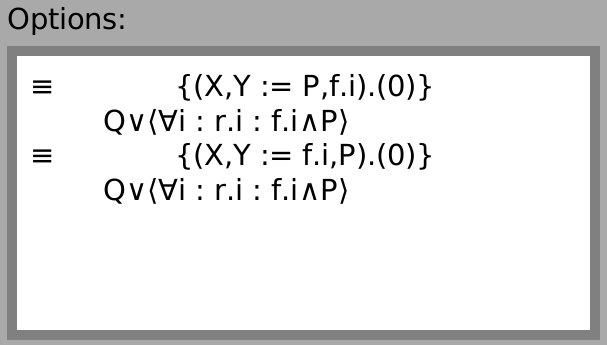
\includegraphics[width=0.4\columnwidth]{optionsgen} 
\end{center}

We choose the first option and the Work Area is updated with the new proof step. We are then free to select a subexpression of the new current expression and continue generating new proof steps until a conclusion has been drawn.

\begin{center}
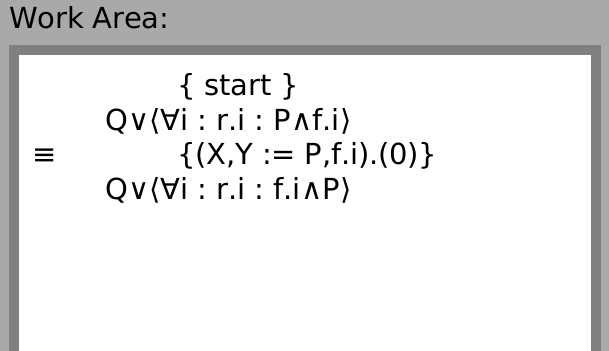
\includegraphics[width=0.4\columnwidth]{newstep} 
\end{center}

If the user is not satisfied with the options and clicks a different theorem, the software will generate a new list of options. This fast cycling and viewing of the options is the strongest point of the Theorem Proving Assistant. It allows easy and fast explorations of different paths during a proof.\\

There are two points to highlight about the generation of options. Firstly, note that the equivalance character is given with the hint, meaning that the current expression and the new generated expression are equivalent. This "transition" character is yielded from the rule. If the rule stated that $[X \wedge Y \Rightarrow Y \wedge X]$ then the transition character would be $\Rightarrow$. There is also a subltly taken into consideration with non-commutative transition characters, such as implication, where depending on the side of the rule which is used, the transition character must be pointing the correct direction. Below is the list of options generated from the given hypothetical theorem.\\

\begin{center}
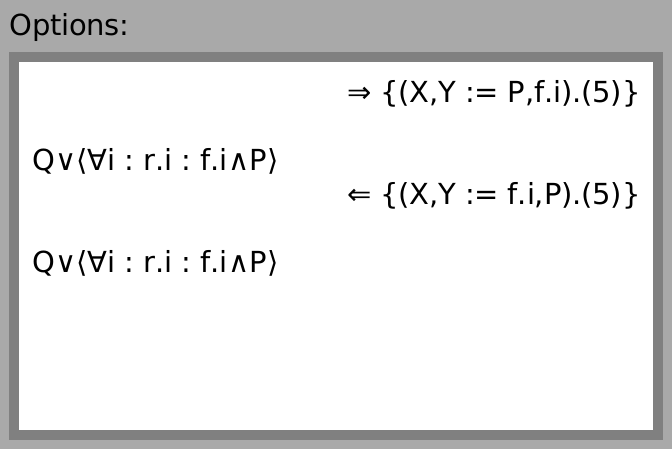
\includegraphics[width=0.4\columnwidth]{imppointing} 
\end{center}

The second point to hightlight is regarding unaccounted for Identifiers. Consider an example where the selection is $true$ and the user wishes to use the rule $[X \equiv X \equiv true]$. It is clear that the replacement is $X\equiv X$ but the replacements $P\equiv P$ and $Q \equiv Q$ are equally valid. Should this case arrise the user is prompted with a dialog to enter the desired mapping.

\begin{center}
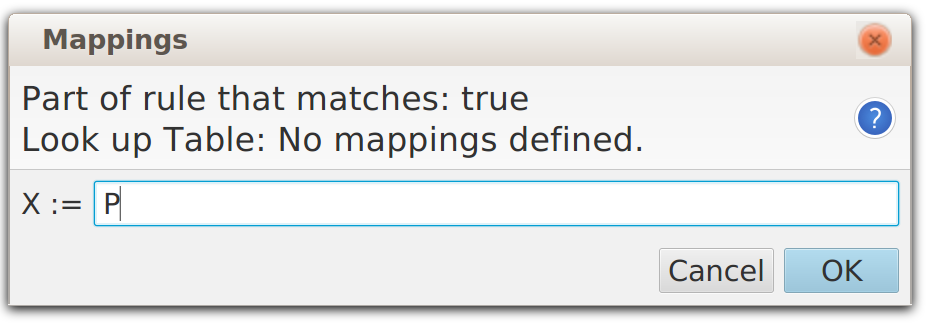
\includegraphics[width=0.55\columnwidth]{mappingpromt} 
\end{center}
\newpage

\end{description}

\end{homeworkSection}

\begin{homeworkSection}{Keeping a Theorem}
When a conclusion has been drawn such as the proof of Absorbtion.0 $[X \wedge ( X \vee Y ) \equiv X]$ the user can save this theorem for future use. The Work Area below shows the entire proof.

\begin{center}
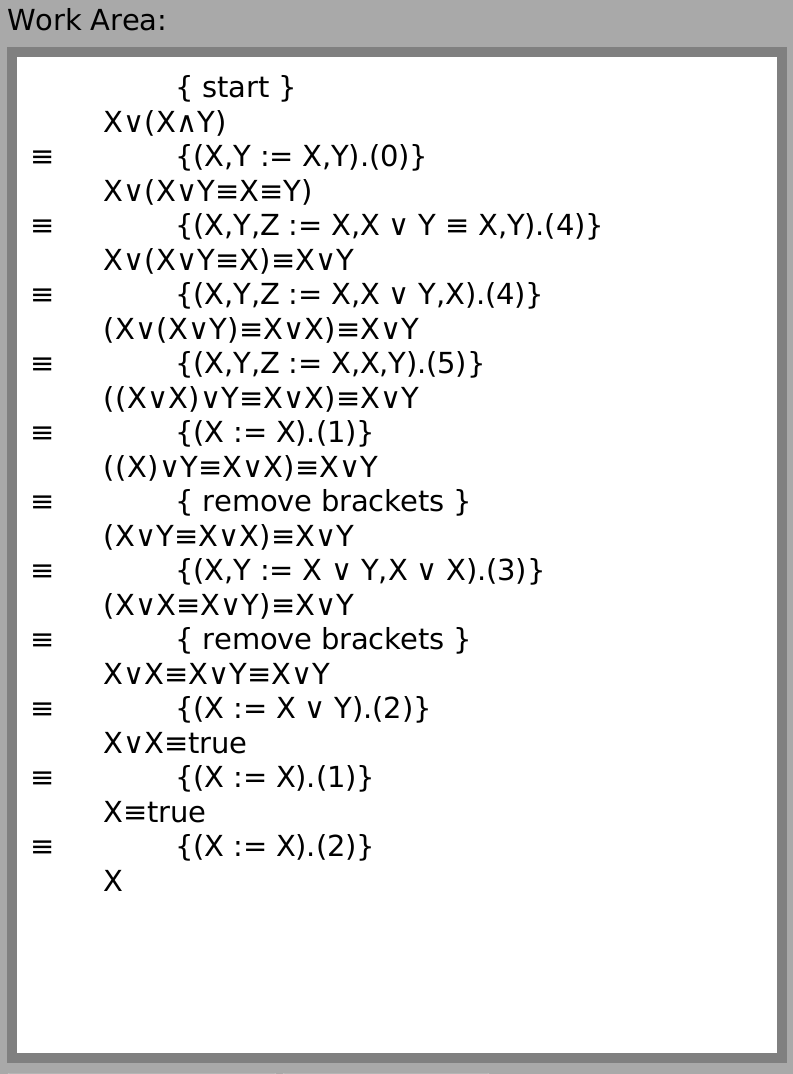
\includegraphics[width=0.4\columnwidth]{absoneproof} 
\end{center}

After clicking the Keeper button the theorem is added to the list of theorems. Note that the equivalance operator ($\equiv$) is used to join the left and right sides of the theorem. If an operator of higher precedence was used within the proof as a transition character, such as implication, then that operator would be used to join the two sides.

\begin{center}
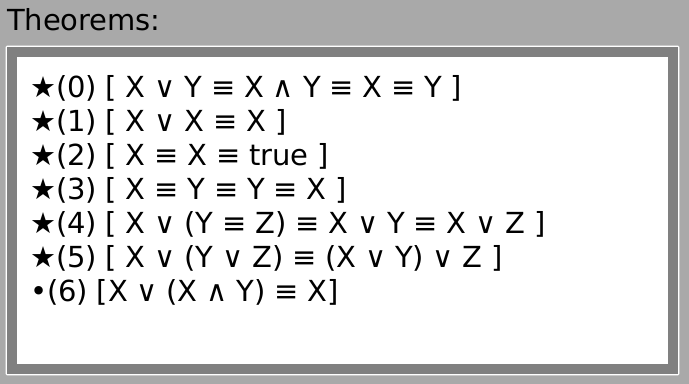
\includegraphics[width=0.4\columnwidth]{keepingabs1} 
\end{center}

The new theorem has been added to the list of theorems and marked with a dot. This indicates that this theorem was proved and was not a given axiom.
\newpage
This kept theorem can be clicked on to be explored. (This feature is only available when the work area is clear). This exploration shows all the proof steps that were taken when proving the theorem. 
\begin{center}
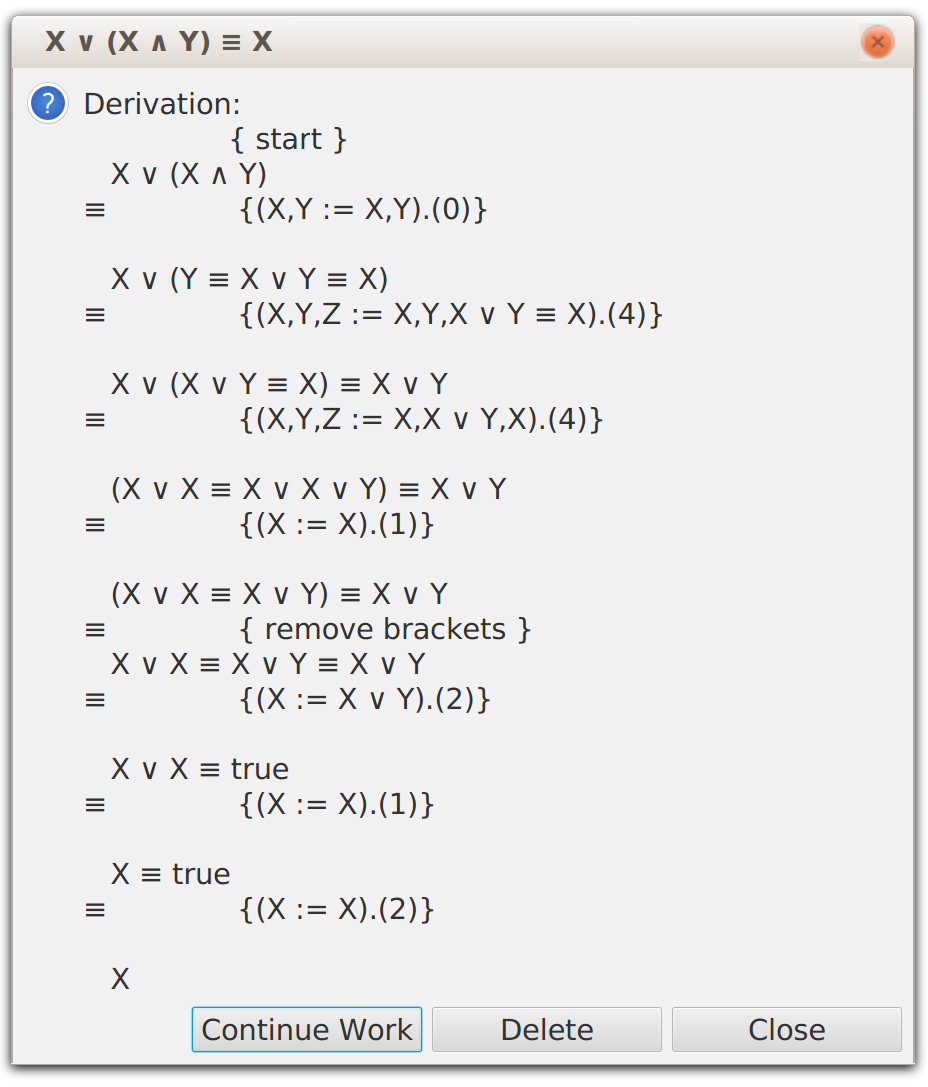
\includegraphics[width=0.55\columnwidth]{abs1derv} 
\end{center}
There is also the option to delete the theorem or to continue work. If Continue is chosen a list of continuation proof steps are given as options. These options are the theorem split up on the lowest precedence operator in the theorem.  
\begin{center}
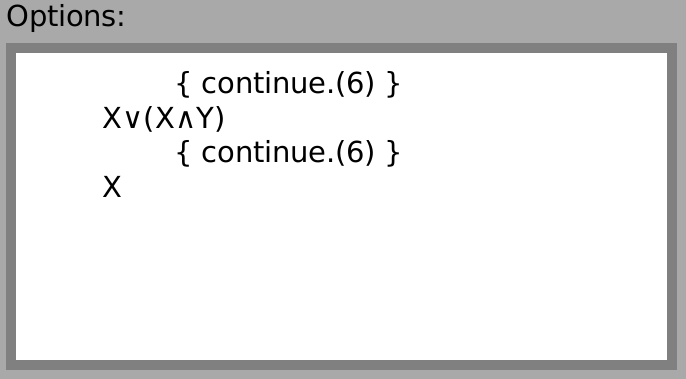
\includegraphics[width=0.4\columnwidth]{abscontinue} 
\end{center}

\end{homeworkSection}
\begin{homeworkSection}{Saving all Theorems}
If the user chooses to save the theorem set the theorems are turned to plain text by googles GSON package. This creates a JSON string for each theorem. The saved theorem file (consisting of JSON strings) can be extended with plain text theorems if needed.
\newpage
\end{homeworkSection}


\end{homeworkProblem}

%----------------------------------------------------------------------------------------

\begin{homeworkProblem}[Backend Algorithms - The Engine]

The software apparently is string manipluation based but the engine driving the system only generates these strings at the moment they are needed. The backend engine has most of the responsiblity of allowing the user to make selections, match them in rules and perform replacements. \\

Here the fundamental methodolgies and algorithms of this engine are discussed.

\begin{homeworkSection}{Expression Representation}

When starting this project the only fact that was clear was the need to not represent expressions as strings. Immidiate issues associated with a string based solution are the lack of sense of precededence, the lack of pivots to easily commute around and no easy way to identify the begining and end of bracketed sections. \\

Syntax trees are a commonly used solution \cite{ULLMAN:1986}. Leaves are identifiers and nodes operators. Below is presented an example with a simple boolean expression: $X\wedge Y \equiv Z$.\\

\Tree [.$\equiv$  [ X Y !{\qbalance} ].$\wedge$ Z ]\\

In order to yield the boolean expression from the tree we need only to perform an in-order travesal, printing the leaf or node's identifier or operator as we visit them. As a human we can read the expression from the tree by reading the identifiers and operators from left to right.\\

Depth is used to indicate precedence. One can see how precedence is maintained as the conjunction operator is at a deeper level than the equivalence. The two operators are commutative and swapping the left and right children of either node will yield an equivalent (in terms of ultimate value) tree. \\

Bracketing sections proved to be more of an issue. Below I demonstrate several options that were considerd with the boolean expresion $(X \wedge Y) \vee Z$. \\

\Tree [.$\vee$ [  [ ( ].X [ ) ].Y  !{\qbalance} ].$\wedge$ Z ]
\Tree [.$\vee$ [ (X Y) !{\qbalance} ].$\wedge$ Z ]
\Tree [.$\vee$ [ [ X Y !{\qbalance} ].$\wedge$ ].$()$ Z ]\\

The decision as to which option to use was implicitly made when attempting to define a valid substring.
\newpage
\end{homeworkSection}

\begin{homeworkSection}{A Valid Sub-expression}
A valid sub-expression is a fundamental part of the project. It is what a user will first select in order to carry out a replacement. For a sub-expression to be valid when selecting it we must respect precedence, bracketing and the number of operands associated with an operator. These requirements indicate that maybe a formal grammar will need to be defined with a corresponding parser but this was avoided as having the ability to parse strings lends its self to string based solutions. The engine needs to work with purely tree based solutions due to the previously discussed issues associated with string manipulation.\\ 

To demonstrate valid and invalid sub-expressions of $X \wedge Y \equiv Z$ I present the table below. 

\begin{center}
\begin{tabular}{|c|c|}
\hline
Valid & Invalid \\
\hline
$X \wedge Y $ & $Y \equiv Z$\\
$X $ & $\wedge Y$\\
$Z $ & $ \equiv Z $\\

\hline
\end{tabular}
\end{center}


Validating the selection of a sub-expression has to be a simple task. Examining drawn syntax trees makes it clear that any node's subtree is a valid sub-expression. For this reason the right most bracket option is used throughout. Any node of that tree can be selected and its subtree is a valid sub-expression. We list the valid sub-exressions of $(X \wedge Y) \vee Z$ beside the tree and the corrolation becomes clear.

\begin{multicols}{2}


\Tree [.$\vee$ [ [ X Y !{\qbalance} ].$\wedge$ ].$()$ Z ]\\
\begin{tabular}{|c|}
\hline
$(X \wedge Y) \vee Z$\\
\hline
$(X \wedge Y) \vee Z$\\
$(X \wedge Y)$\\
$X \wedge Y$\\
$X$\\
$Y$\\
$Z$\\
\hline
\end{tabular}

\end{multicols}


Initially this simple approach of using a node's subtree to define a sub-expression appeared comprehensive but when attempting to extract all valid sub-expressions of an expression with associative operators it became clear that this was not possible. We use the expression $X \wedge Y \wedge Z$ to demonstrate this. Consider the following tree representation and list of valid sub-expressions as defined above.

\begin{multicols}{2}

\Tree [.$\wedge$ [ X Y !{\qbalance} ].$\wedge$ Z ]\\
\begin{tabular}{|c|}
\hline
$X \wedge Y \wedge Z$\\
\hline
$X \wedge Y \wedge Z$\\
$X \wedge Y$\\
$X$\\
$Y$\\
$Z$\\
\hline
\end{tabular}

\end{multicols}

$Y \wedge Z$ is a valid sub-expression of $X \wedge Y \wedge Z$ but is not attainable from the above tree in its current state. We need to permute the syntax tree to "re-shuffle" it so $Y \wedge Z$ can exist as a subtree while still maintaining the value of the boolean expression. 

\newpage
\end{homeworkSection}
\begin{homeworkSection}{Permutations of a Syntax Tree}

In order to achieve this re-shuffling of a tree we need to rely on a tree rotation algorithm called zigging \cite{GOODRICH:2010}. Performing the zig operation on the deeper conjunction node will rotate the tree clockwise, causing the node to be the new root. $X$ will be the left child of the new root with the previous root as its right child. The old roots right child, $Z$, persists, and the temporarily orphaned $Y$ becomes $Z$s sibling. The following two trees present two permutations of a tree for $X\wedge Y\wedge Z$ attainable by zigging the left or right child of the root.

\Tree [.$\wedge$ [ X Y !{\qbalance} ].$\wedge$ Z ] 
\Tree [.$\wedge$  X [ Y Z !{\qbalance} ].$\wedge$ ]\\

Now by unioning the the set of sub-expressions yielded from the two trees we have a complete set. This simple approach however does not scale. An algorithm combining zigging nodes and zigging nodes from a depth of two is needed in order yield all valid sub-expressions of any tree. \\

Consider the following series of tree representations of $X \wedge Y \wedge Z \wedge W \wedge Q$ and one can see how the whole tree is being "dragged" through the root node by performing the zig operation on the roots left child.

\Tree [ .$\wedge$ [ [ [ X Y !{\qbalance} ].$\wedge$  Z ].$\wedge$ W  ].$\wedge$ Q ] 
\Tree [ .$\wedge$ [ [ X Y !{\qbalance} ].$\wedge$ Z ].$\wedge$ [ W Q !{\qbalance} ].$\wedge$ ]\ \ \ \ 
\Tree [ .$\wedge$  [ X Y !{\qbalance} ].$\wedge$ [ Z [ W Q !{\qbalance} ].$\wedge$ ].$\wedge$ ] 
\Tree [ .$\wedge$ X [ Y [ Z [ W Q ].$\wedge$ ].$\wedge$ ].$\wedge$ ]\\

After each zig we add a copy of the tree as it stands to a set and continue until no new trees are generated. This we will ultimately create every possible permutation. When the alorithm stops we have will yielded all equivalent tree permutations. The following tree is one of them which will be produced at some point during permuting algorithm.

\Tree [ .$\wedge$ [ X Y !{\qbalance} ].$\wedge$ [ [ Z W !{\qbalance} ].$\wedge$ Q ].$\wedge$ ]\\

When attempting to identify valid sub-expressions of an expression all permutations of that expressions's tree must exist simulatiously. All possible tree arrangments for a given expression must be considered when validating or refuting an operation on an expression.


\newpage
\end{homeworkSection}
\begin{homeworkSection}{Matching, Mapping and Replacing}

At this point a new theorem must be introduced but no longer in terms of X and Y but P and Q.
\begin{align*}
&\cdot\ \ [P \wedge ( P \vee Q ) \equiv P]& absorbtion0
\end{align*}
We consider a state half way through a proof where the user's current expression is $X \wedge (X \vee Y ) \equiv X \wedge Y$ and wishes to use absorbtion0 to replace the entire left hand side of the expression with X. The action is documented below with the notation we defined.
\begin{align*}
&X \wedge (X \vee Y ) \equiv X \wedge Y  \\
=&\dent \{(P,Q\coloneqq X,Y).(absorbtion0)\}\\
&X \equiv X \wedge Y
\end{align*}

As humans we can easily map P to X and Q to Y and do the replacement as it is in our nature to look for patterns and repetition. To design alorithms for a computer to do this is an complex task. To further complicate the matter we change the the boolean identifier Y on the left hand side of the expression to a boolean expression consisting of several operands. We redine the current expression and application of absorbtion0 as follows.
\begin{align*}
&X \wedge (X \vee (Z \wedge W) ) \equiv X \wedge Y  \\
=&\dent \{(P,Q\coloneqq X,(Z \wedge W)).(absorbtion0)\}\\
&X \equiv X \wedge Y
\end{align*}

In looking to match the users selection ($X \wedge (X \vee (Z \wedge W) )$) with a sub-expression of absorbtion0 we must compare it to every valid sub-expression of absorbtion0. Not only that, but we must handle the fact that the boolean identifiers in the rule and current expression are completely different. We start by drawing a tree representation of the current expression with the current expression highlighted and the rule, absorbtion0. Note that I have convieniently chosen to draw the correct permutation the rule. The software program actually itterates through all permutations in attempts to find matches. \\

Current Expr:
\Tree[ .$\equiv$ [ X [ [ X [ [ Z W !{\qbalance} ].$()$ ].$\wedge$ ].$\vee$ ].$()$ ].$\wedge$ !{\qframesubtree} [ \ X Y !{\qbalance} ].$\wedge$ ]
Absorbtion0:
\Tree[ .$\equiv$ [ P [ [ P Q !{\qbalance} ].$\vee$ ].$()$ ].$\wedge$ P ]\\

The matching algorthim first requests all valid trees representing the rule with a root node that was a child of an equival node and has an operator which matches the root of the selection. In this case, the single permutation of the subtree which starts at absorbtion0's single conjunction operator.\\

We walk each of the yielded subtrees along side the current selection tree checking equivalence at each step. If a discrepency is found (such as operators that don't match) that subtree is discarded and we examine the next. During the walk if an identifier is found in the rule's subtree, that identifier is added to a look-up table with the corresponding node from the selection. This lookup table will define the mapping used in the hint.\\

During the walk of the example trees provided there are three identifiers to be found in the subtree of  absorbtion0.
\begin{enumerate}
\item On discovery of P (the left child of the subtrees root), it will map directly to the corresponding X in the current expresion. $P \rightarrow X$ will be added to the look up table.
\item On discovery of the second P we must be sure that this new mapping we are about to define corresponds with the mapping defined in step 1. If there is a discrepency this permutation of the subtree of the rule is not valid and thus discarded.
\item On discovery of the identifier Q we note that it does not correspond to another identifier, but a whole expression. That is not a problem and we add $Q \rightarrow (Z \wedge W)$ to the look-up table.
\end{enumerate}

If the walk of any subtree of the rule that is checked completes, then we add that subtree and its look-up table to a list. This list will be the list of possible uses of a rule on a selection. Be aware that there may be multiple uses of a rule on a selection. In the example given the list will contain only one element, the following subtree and lookup table. One final check needs to be carried out to determine if there is a variable in the rule which has no baring on the selected sub expression, ie: it has no mapping automatically defined. In this case the mapping is open, and any value can be chosen.
\begin{multicols}{2}
\Tree [ .$\wedge$ P [ [ P Q !{\qbalance} ].$\vee$ ].$()$ ] \\
\begin{tabular}{|c|}
\hline
Look-Up Table\\
\hline
$P \rightarrow X$\\
$Q \rightarrow (Z \wedge W)$\\

\hline
\end{tabular}

\end{multicols}

To complete the replacement step there are a few small steps to take. None of which pose a large issue. We now need to remove the subtree from the permutation of the rule that contained it. In this case it will leave just the P node. Once we have the rule without the matched subtree we need to walk it and use the lookup table to replace its identifiers with their new nodes.\\

In this example the rule without the matching subtree, P, will be walked and have its node replaced with its counterpart from the lookup table, X. At this point the matching and mapping is complete and we can return to the original expression we were working on and replace the current selection with the new tree (in this case, just an identifier node).\\

\Tree[ .$\equiv$ X !{\qframesubtree} [ \ X Y !{\qbalance} ].$\wedge$ ]

The replacement step has been performed, we know what rule we used and we also know what assignemnts were made into the rule. We can use this information to generate the needed hint and present the user with the outcome they expect. Here the replacement step from the start of this section is presented again to conclude the calculation of the step.
\begin{align*}
&X \wedge (X \vee (Z \wedge W) ) \equiv X \wedge Y  \\
=&\dent \{(P,Q\coloneqq X,(Z \wedge W)).(absorbtion0)\}\\
&X \equiv X \wedge Y
\end{align*}

\newpage
\end{homeworkSection}


\end{homeworkProblem}

%----------------------------------------------------------------------------------------
\begin{homeworkProblem}[Frontend Algorithms - The User Interface]
Two major alrogithms were needed to link the backend engine with the graphical user inteface. Before introducing them the term "bit" must be introduced. In this context a bit referes to a character displayed to the user. A bit has many subtle properties which allow the software to perform. A further extenstion of this is the notion of a Bit Box. The software is impletmented with JavaFX, and the container used to house an entire expression is a HBox (horizontal box) so they are refered to as Bit Boxes.

\begin{homeworkSection}{The Bit Box Maker}
To give the illusion of a string based piece of software a Bit Box is used to house an expression. For expressions with no bracket-type (brackets or floor/ceiling) or unary operators. a simple in-order traversal of any one of the trees for an expression will suffice. One only needs to create a bit when visiting each node with a corresponding character and add it to the Bit Box. \\

If a bracket-type node is found during the traversal then two bits need to be created, the opening and closing bits. In this case the open bit inserted before continuing the traverse. Only when the recursive tree walker returns to to the level of this bracket-type node is the closing bit inserted. It can be thought of a special case "pre \& post" order traversal.\\

In the case of a unary operator such as negation the node is simply visited, and a bit added to the Bit Box, before continuing to traverse. It is treated as a pre-order visit. Both of these exceptions are special cases that are handled by the tree walker.


\end{homeworkSection}

\begin{homeworkSection}{The Associator} 

It is the role of the Associator to associate bits and their corresponding nodes in the syntax trees. It is not a bijective mapping as one bit can map to many nodes in equivalent (in terms of the expression they represent) syntax trees. Each bit has a list of nodes with which it is associated. Should the bit belong to a bracket-type node then it has a "bracket-buddy". This is a reference to the corresponding closing (or opening) bracket. Only one of these two will hold the list of bracket-type nodes.\\

Each equivalent syntax tree is walked and the bits itterated across. The bits lists of nodes are populated. Bracket-type nodes and Unary nodes have to be handled carefully as they break the ordering of the in-order traversal. Instead of using convoluted logic to track the locations of these bits they are simply pushed onto a stack. Similary, any opening bracket-type bit is pushed onto a parralel stack. Closing bracket-type bits are skipped as they are not needed, the bracket-buddy reference is used instead. After completion of the walk of each tree and single itteration of the bits, (which conclude at the same time), we have two sets of stacks. One for bracket-type operators with a bit stack and a node stack, and another for unary operators with same. The bit and Node stacks are popped in tandem and associated as their order in the stacks correspond. \\

The nodes and bits are associated in this way so that when a user clicks on any bit, it is known what valid sub expressions that bit is a root of as it has a reference to that root. We need only walk that sub tree and hightlight each bit associated with the visited nodes in order to hightlight, and thus select, a valid subexpression. Repeatedly clicking on the same bit will cycle the subtrees with which is it associated and hightlight different subexpressions.
\newpage
\end{homeworkSection}

\end{homeworkProblem}
%----------------------------------------------------------------------------------------
\begin{homeworkProblem}[The Parser and Grammar]
In order to start theorems the user needs to type in a starting expression. For simplicity, A plain text psuedo language was defined (see Appendix A) with which a user can specify the starting expression. A lexer uses a string tokenizer to itterate throught the input symbols and then a recursive descent parser (RDP) builds the abstract syntax tree for the expression (assuming it's valid).\\

\begin{homeworkSection}{The EBNF Grammar}
In order to build an RDP a grammar was needed. JJTree and JavaCC were considered as a tools to build an RDP but ultimately it was deemed too heavy weight. A grammar was defined in extended Backus–Naur form (EBNF) (see Appendix B). The EBNF grammar consits of terminal symbols and non-terminal production rules. The terminal symbols define legal characters and strings in the expressions and the non-terminal production rules define the way in which the symbols can be legally arranged in order to create expressions. 
\begin{itemize}
\setlength\itemsep{0em}
\item Terminal symbols are enclosed in angle brackets ($<>$) and have a sequecnces of characters associated with them. Eg: $<$ID$> \coloneqq$  [A-Z,a-z]+
\item Production rules have a left hand side and a right hand side. The left hand side is a non-terminal and the right hand side is a combination of terminals and non-terminals.\\
Eg: Max $\coloneqq Val \{ \uparrow Val\}$ (where val produces a terminal)\\
The \{ and \} brackets indicate an optional amount of the terminals and non terminals within it. This allows for arbirtrarily long expressions with the Max operator. \\
Alternate production rules are indicated with a $|$.
\end{itemize}

The entire grammar is documented in Appendix B.

\end{homeworkSection}

\begin{homeworkSection}{The Parser}
The parser has two key roles; to build the syntax tree for the expression and to respect the laws of precendence of the operators while doing so. To build the parser I followed a very simple approach of defining a method for each non-terminal production. The order in which these methods are called is the order of precedence of the operators. Each method follows the same framework. Except for the final method, factor(). The factor() method has special code to define the different types of node to create, depending on the value yielded by the lexer.\\
Below is one of the standard methods. Seeing as or() is called from within implication() it will cause disjunction expressions to be created at a deeper level in the tree, and as a result the disjunction operator will be considered to have a higher precedence than that of implication.

\begin{lstlisting}
    public void implication() {
        or();
        while (symbol == Lexer.IMPLICATION) {
            INode n = new BinaryOperator(Operators.IMPLICATION, null, null);
            n.children()[0] = root;
            or();
            n.children()[1] = root;
            root = n;
        }
    }
\end{lstlisting}

Using this RDP will ensure that any legally constructed expressions, written in plain text, will yield a syntax tree which respects the precedence of the operators. This is essential for the algorithms in the engine of the Theorem Proving Assistnant to work.
\end{homeworkSection}

\newpage

\end{homeworkProblem}
%----------------------------------------------------------------------------------------
\begin{homeworkProblem}[Design Details and Implementation]

\begin{homeworkSection}{Tools Used}
\begin{description}
\item \textbf{Java}\\
The Theorem proving assistant is almost exclusively written in Java. It must be compiled and exectuted with Java 1.8 or greater. Java was chosen for several reasons.
\begin{itemize}
\setlength\itemsep{0em}
\item High portability of written applications.
\item Multiple inheritance allowes nodes to be given characteristics. When walking trees it is essential to be able to identify the abilities of a node. For example, all of the terminal classes (ArrayAndIndex, Identifier, Literal and QuantifiedExpression) implement INode and ITerminal.
\item A wide variety well documented of libraries exists such as JavaFX and GSON.
\item Memory managment is automatic. Attempting to manange the allocation and deallocation of the trees in this piece of software would prove very challenging. When permuting an expression hundreds of instances of nodes are created and de-referenced. The garbage collector handles the memory de-allocation of these de-referenced nodes automatically.
\end{itemize}
\item \textbf{JavaFX}\\
When attempting to decide on the platform for creating the application Java Swing was initially considered. JavaFX is intended to replace the Java Swing library and seeing as its API is much cleaner and easier to work with it was chosen as the platorm on which to build the Theorem Proving Assistant. For example, JavaFX takes care of alot of the mandatory code automatically such as redrawing the application after an update. JavaFX also supports CSS styling which is the other language used to develop with. (All 17 lines of it!).
\item \textbf{GSON}\\
In order to save and load theoremsm initially a plain text approach was taken but the need for more information than just the expression was needed, such as a theorems derivation string. Google's GSON library was used to turn Java data-bean objects to JSON strings for saving theorem sets, and JSON strings to Java objects for loading theorem sets.
\item \textbf{JUnit4}\\
JUnit is a unit testing framework for Java. Throughout this project it was used for regression testing to maintain the integrety of current features while adding functionality.
\item \textbf{IntelliJ}\\
IntelliJ is a market leading IDE. As a student the commercial version is available for free. It was chosen due to it's ability to generate needed code quickly and automatically as well as its very powerful refactoring tools. At one stage in the development process alot of Lists to had to be migrated to Sets. IntelliJ made this very easy, automatically migrating effected methods, fields and variables.
\item \textbf{Git and GitHub}\\
Git's version control system facilitated the exploratory approach to building this software package. New features were developed on their own branch and only when the feature was fully tested and correct was it merged into the master branch. Several branches were abandoned during the development process, reverting back to the master branch (at an earlier point in time) to start an entirely different approach.\\

Github was used to back up the code base regularly and to share my code and application with others. Peers regurlary provided 3rd party functionality unittesting and gave good feedback which influenced some design decisions.

\end{description}
\newpage
\end{homeworkSection}

\begin{homeworkSection}{Class Diagrams}
The Theorem Proving Assistant consists of thirty seven Java classes across thirty six files. While it is possible to generate a diagram of the entire application it's so large it would offer no benefit. Instead three small subsets of the diagram are presented here.\\

\begin{description}
\item \textbf{The Backend Engine}\\
The entry point to the engine is the Replacer class. It is the responisibility of this class, when given an expression, a selection and a rule, to yield possible replacement options. It directly relies on four other worker classes and indirectly on three data-bean classes.
\begin{center}
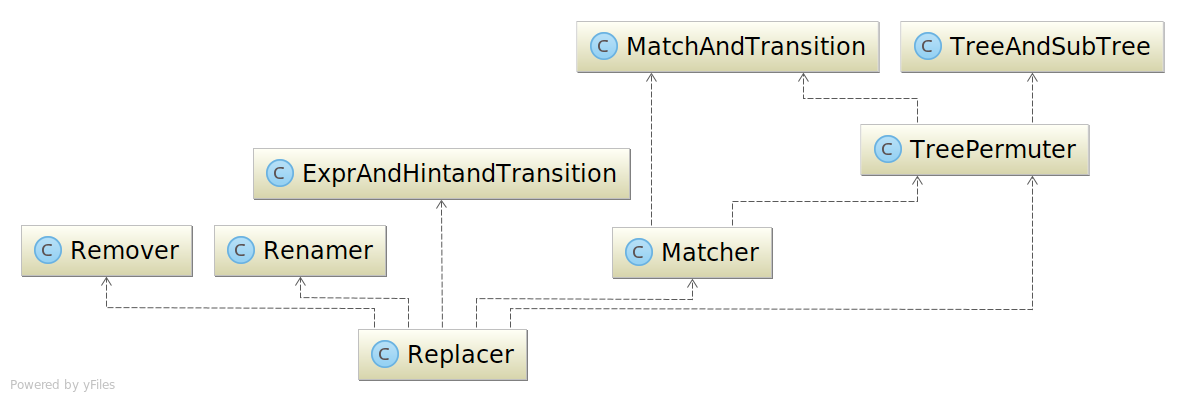
\includegraphics[width=0.77\columnwidth]{../uml/workers2} 
\end{center}

\item \textbf{The Front End GUI}\\
The TheoremProvingAssistant class is the entry point of the Gui. Any class preappended with CL is a click listener. The theorem click listener has a Replacer which is called upon to yield valid replacements.\\

The State class in the top left maintains the state of the application. References to values such as the current expression, the list of theorems available and the steps in the current proof are all available through this class. It is not a manager as it has no logic code, it merely holds references to values.\\

The Associator and BitBoxMaker classes can be seen depending on the Bit class in order to create a ProofStep. Both the TheoremProvingAssistant and TheoremLoader classes depend on the Parser to build syntax trees.
\begin{center}
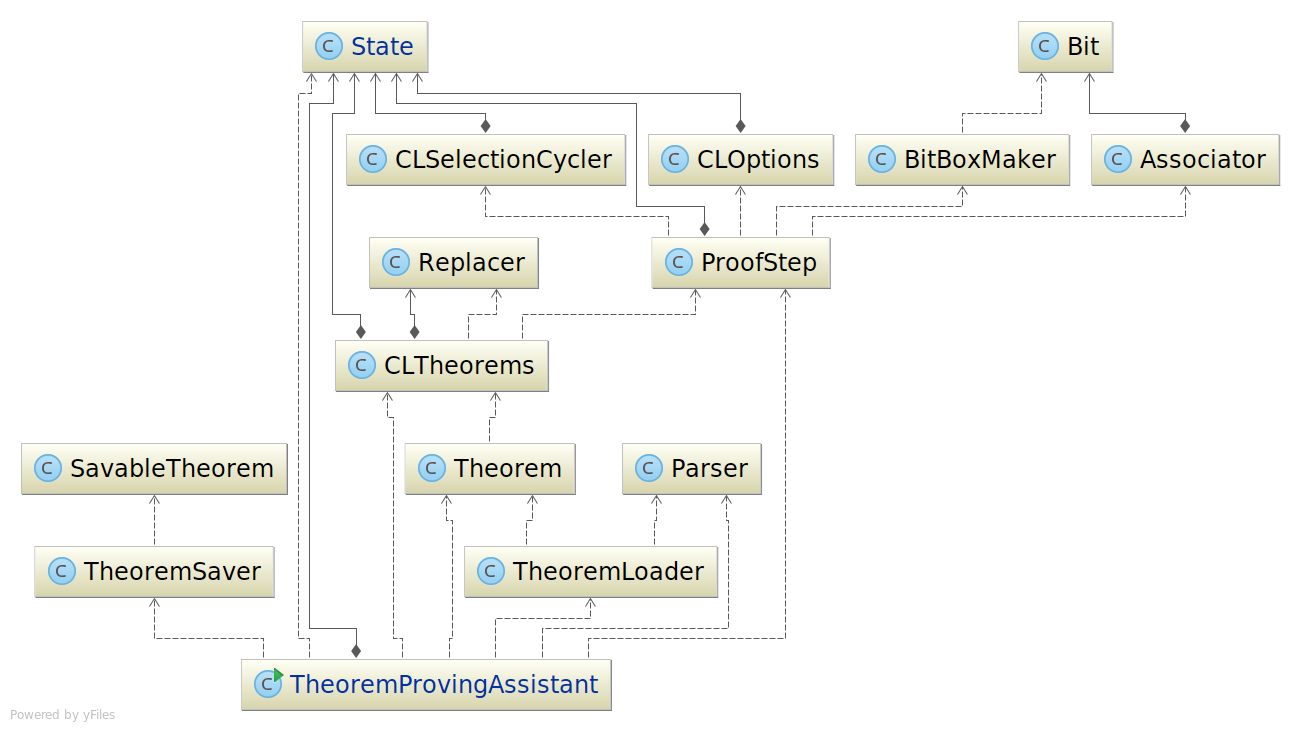
\includegraphics[width=0.86\columnwidth]{../uml/GUIFive} 
\end{center}
\newpage

\item \textbf{The Parser}\\
It is the role of the Parser class to create syntax trees. These trees consists of Operators and Terminals. Code which is common to all nodes is implemented in the Node class, a superclass of the specific nodes.\\

Each non bracket-type node class implements either ITerminal, IUnaryOperator or IBinaryOperator. It is with these interfaces that the classes can be refereneced polymorphically. For the same reason, although it is not displayed here for clarity, every class which is used as a node implements INode. 
\begin{center}
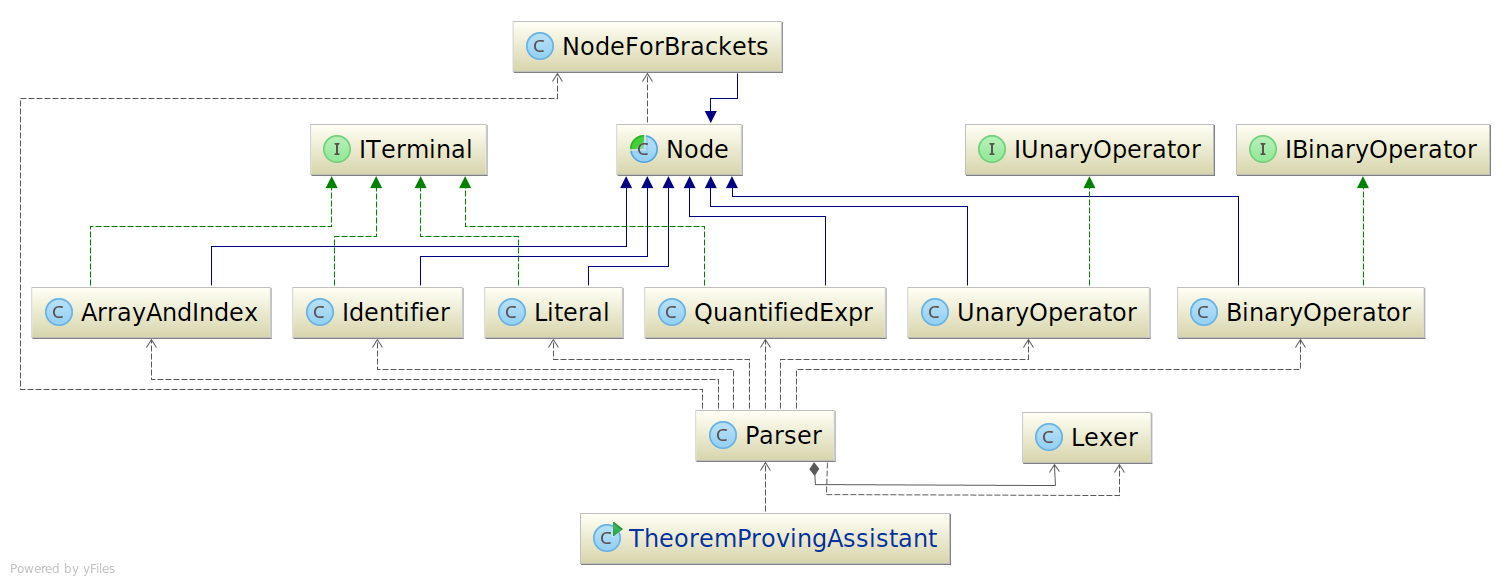
\includegraphics[width=1\columnwidth]{../uml/parser3} 
\end{center}

\end{description}

\newpage
\end{homeworkSection}

\end{homeworkProblem}


%----------------------------------------------------------------------------------------
\begin{homeworkProblem}[Testing And Evaluation]

Throught the build process it was important to maintain a suite of unit tests to verify the integrity of features as work continued. It is needed to know that being relied upon in a black-box manor is still functioning as expected. This type of testing is known as regression testing. It increases the chances of bugs being detected throughout development.

\begin{homeworkSection}{Regression Testing}
For every new calculus, feature, worker developed a test was written, some times multiple. These tests were packaged into three major suites:
\begin{description}

\item \textbf{Tree Test}\\ 
The trees are the core of this project. It is needed to know that they are being walked and read correctly. This suite of tests walks and prints the characters in an in-order traversal (with the exception of bracket-type and unary operator nodes) and compares the output with an expected corresponding string.
\item \textbf{Worker Tests}\\ 
The worker tests were the most important tests. Throught the build process the workers were treated as black-boxes. Their implementation wasn't known and they were relied upon to provide consistantly valid results. Often the addition of some function to a worker resulted in tests failing in another. Maintaining a fully passing test suite enabled a very desirable black-box style of programming.
\item \textbf{Misc Tests}\\ 
These test were for testing small independant features of the application such as the tree copying logic aswell as testing the indiviual components of a quantified expression.

\end{description}
\end{homeworkSection}

\begin{homeworkSection}{Complexity Testing}
The Theorem Proving Assistant pivots around the tree permutation algorithm where nodes of a syntax tree representing an expression are zigged in order to yield all trees which represent that expression. An extention of this algorithm yields all valid sub-expressions of an expression. The worst case complexity of both is calculated here.
\begin{description}
\item \textbf{Yield All Trees For an Expression}
\begin{align*}
X&=Y
\end{align*}
\item \textbf{Yield All Valid Subexpressions}
\begin{align*}
Y&=X
\end{align*}
\end{description}
\end{homeworkSection}

\begin{homeworkSection}{Proving Correctness}
The regression testing is needed to verify that that algorithms are working as expected. Proving correctness of the software is an entirely different process. Here a case study over the boolean calculus is presented.
\newpage
\end{homeworkSection}
\end{homeworkProblem}

%----------------------------------------------------------------------------------------

\begin{homeworkProblem}[Conclusion]

\begin{homeworkSection}{Progress So Far}
It's done
\end{homeworkSection}

\begin{homeworkSection}{Further Work}
Pffft
\newpage

\end{homeworkSection}


\end{homeworkProblem}


%----------------------------------------------------------------------------------------

\begin{homeworkProblem}[Appendix]

\begin{homeworkSection}{The Plain Text Pseudo-Language}
\begin{description}
\item \textbf{Boolean Expressions}\\
$X \equiv Y$: \texttt{"X == Y"}\\
$X \not\equiv Y$: \texttt{"X !== Y"}\\
$X \wedge Y$: \texttt{"X and Y"}\\
$X \vee Y$: \texttt{"X or Y"}\\
$X \Rightarrow Y$: \texttt{"X -> Y"}\\
$X \Leftarrow Y$: \texttt{"X <- Y"}\\
$\neg X$: \texttt{"! X"}\\
$X \wedge ( Y \vee Z )$: \texttt{"X and ( Y or Z )"}

\item \textbf{Quantified Boolean Expressions}\\
$\langle \forall i : r.i : f.i \rangle$: \texttt{"<| forall i : r.i : f.i |>"}\\
$\langle \exists j : s.j : g.j \rangle$: \texttt{"<| exists j : s.j : g.j |>"}

\item \textbf{Floor/Ceiling Expressions}\\
$\lfloor x \rfloor$: \texttt{"|\_ x \_|"}\\
$\lceil x \rceil$: \texttt{"|\fontencoding{OT1}\selectfont\symbol{13} x \fontencoding{OT1}\selectfont\symbol{13}|"}\\
$\lfloor x \rfloor \leq x$: \texttt{"|\_ x \_| <= x"}\\
$\lceil x \rceil \geq x $: \texttt{"|\fontencoding{OT1}\selectfont\symbol{13} x \fontencoding{OT1}\selectfont\symbol{13}| >= x"}\\
$\lfloor x + n \rfloor = \lfloor x \rfloor + n$: \texttt{"|\_ x + n \_| = |\_ x \_| + n"}\\

\item \textbf{Lattice Theory Expressions}\\
\resizebox{0.97\hsize}{!}{$\langle \forall x,y :: x \sqsubseteq y \wedge y \sqsubseteq x \Leftarrow x=y \rangle$: \texttt{"<| forall x,y : : x under y and y under x <- x = y |>"}}\\
\resizebox{0.97\hsize}{!}{$\langle \forall z :: x \sqsubseteq z \equiv y \sqsubseteq z \rangle \Rightarrow x=y $: \texttt{"<| forall z : : x under z == y under z |> -> x = y"}}

\item \textbf{Max/Min Expressions}\\
$x \uparrow y$: \texttt{"x up y"}\\
$x \downarrow y$: \texttt{"x down y"}

\end{description}


\newpage
\end{homeworkSection}

\begin{homeworkSection}{The Grammar}


\begin{verbatim}
Expr := NotEq { <EQUIV> NotEq }
NotEq := Impl { <NOT_EQUIVAL> Impl }
Impl ::= FF { <IMPL> FF }
FF ::= Or { <FF> Or }
Or ::= And { <OR> And }
And ::= Equals { <AND> Equals }
Equals ::= NotEquals { <EQUAL> NotEquals }
NotEquals ::= Lt { <NOT_EQUALS> Lt }
Lt ::= Gt { <LT> Gt }
Gt ::= Lte { <GT> Lte }
Lte ::= Gte { <LTE> Gte }
Gte ::= Over { <GTE> Over }
Over ::= Under { <OVER> Under }
Under ::= Up { <UNDER> Up }
Up ::= Down { <MAX> Down }
Down ::= Add { <MIN> Add }
Add ::= Minus { <PLUS> Minus }
Minus ::= Factor { <MINUS> Factor }
Factor ::= <ID> | <NOT> Factor | <LPAR> Expr <RPAR> | <LFLOOR> Expr <RFLOOR>
           | <LCEILING> Expr <RCEILING> | <ARRAY_AND_INDEX>
           | <LANGLE> <EXISTS> <ID> <COLON> Expr <COLON> Expr <RANGLE>
           | <LANGLE> <FORALL> <ID> <COLON> Expr <COLON> Expr <RANGLE>
<EQUIV>  ::= "=="
<NOT_EQUIV>  ::= "!=="
<IMPL>  ::= "->"
<FF>  ::= "<-"
<OR>  ::= "or"
<AND>  ::= "and"
<EQUAL>  ::= "="
<NOT_EQUALS>  ::= "!="
<LT>  ::=  "<"
<GT>  ::= ">"
<LTE>  ::= "<="
<GTE>  ::= ">="
<OVER>  ::= "over"
<UNDER>  ::= "under"
<MAX>  ::= "up"
<MIN>  ::= "down"
<PLUS>  ::= "+"
<MINUS>  ::= "-"
<ID> ::= "[A-Z,a-z]+"
<NOT> ::= "!"
<LPAR> ::= "("
<RPAR> ::= ")"
<LFLOOR> ::= "|_"
<RFLOOR> ::= "_|"
<LCEILING> ::= "|'"
<RCEILING> ::= "'|"
<ARRAY_AND_INDEX> ::= "[A-Z,a-z]+\.[A-Z,a-z]+"
<LANGLE> ::= "<|"
<RANGE> ::=	"|>"
<COLON> ::= ":"
\end{verbatim}
\newpage

\end{homeworkSection}




\end{homeworkProblem}
%----------------------------------------------------------------------------------------


\begin{thebibliography}{99}

\bibitem{DEEPBLUE:1997} http://www-03.ibm.com/ibm/history/ibm100/us/en/icons/deepblue/
\bibitem{PROBFRACT}Dominic Basulto 2016 - http://bigthink.com/endless-innovation/humans-are-the-worlds-best-pattern-recognition-machines-but-for-how-long
\bibitem{DIJKSTRA:1990} Carel S. Scholten and Edsger W. Dijkstra. \emph{Predicate Calculus and Program Semantics}. 220 pages. \\ISBN: 978-1-4612-7924-2. Springer-Verlag New York, 1990.
\bibitem{ULLMAN:1986} Jeffrey Ullman, Alfred Aho, and Ravi Sethi. \emph{Compilers: Principles, Techniques, and Tools}. 796 pages. \\ISBN: 0201100886. Addison Wesley, 1986.
\bibitem{GOODRICH:2010} Michael T. Goodrich and Roberto Tamassia. \emph{Data Structures and Algorithms in Java}. 736 pages. \\ISBN: 978-0-470-39880-7. John Wiley \& Sons Inc, 2010.
\end{thebibliography}

\end{document}